\documentclass[preprint]{vgtc}

\usepackage{times}
\renewcommand*\ttdefault{txtt}
\usepackage{mathptmx}

% *** MATH PACKAGES ***
%% with other math-related packages, you may want to disable it.
\usepackage{amsmath, amsthm, amsfonts,amssymb,eulervm,xspace, mathtools}
\usepackage{stmaryrd}%maps from
%\renewcommand{\restriction}{\mathord{\upharpoonright}} %restriction w/p space
\usepackage{mathrsfs} % math script fonts
\usepackage{relsize} %bigger
\usepackage{bm}

\usepackage{xcolor}
\usepackage{multicol}
\usepackage{notation}
\usepackage{wrapfig}
\usepackage{multirow}
\usepackage{hyperref}
\usepackage{caption}

\usepackage{graphicx}
\usepackage{amsmath,amssymb}
\usepackage{mathtools}
% *** diagrams
\usepackage{tikz}
\usetikzlibrary{cd}
% *** ALIGNMENT PACKAGES ***
\usepackage{tabu}                      % only used for the table example
\usepackage{tabulary}
\graphicspath{{../paper/figures/}{figs}}

\onlineid{0}
\vgtccategory{Research}
%\vgtcinsertpkg




\title{Topological Equivariant Artist Model}

\author{
Hannah Aizenman\thanks{e-mail: haizenman@gradcenter.cuny.edu} \\
\scriptsize{CUNY Graduate Center}
\and
Mikael Vejdemo-Johansson\thanks{e-mail: mvj@math.csi.cuny.edu} \\
\parbox{1.6in}{\scriptsize \centering CUNY College of Staten Island \\
CUNY Graduate Center}
\and
Thomas Caswell\thanks{e-mail: tcaswell@bnl.gov} \\
\parbox{1.8in}{\scriptsize\centering National Synchrotron Light Source II \\ Brookhaven National Lab}
\and
Michael Grossberg\thanks{e-mail: mgrossberg@ccny.cuny.edu} \\
\parbox{1.6in}{\scriptsize\centering City College of New York \\ CUNY Graduate Center}
}

%\keywords{TODO:list keywords}

\abstract{
    The contract data visualization tools make with their users is that a chart is a faithful and accurate visual representation of the numbers it is made from. Motivated by wanting to make better tools, we propose a methodology for fully specifying arbitrary data to visualization mappings in a manner that easily translates to code and provides a consistent interface for accessibility tools to query for information about the state of the visualization. We propose that fiber bundles provide a uniform interface for describing a variety of underlying data - tables, images, networks, etc. - in a manner that independently encodes the mathematical structure of the topology and the fields of the dataset. Modeling the data structures that store the datasets as sheaves provide a method for specifying visualization methods that are designed to work regardless of how the dataset is stored - whether the data is on disk, distributed, or on demand. Specifying the visualization library components as natural transforms of sheaves means that the constraints that the component must satisfy to be structure preserving can be specified as the set of morphisms on the data and graphic sheaves, including the structure on the topology and fields of the data.  Using category theory to formally express how visual elements are constructed means we can translate those expectations into code, which can then be used to enforce the expectation that a visualization tool is faithfully translating between numbers and charts. The sheaf formalism is generic enough that with appropriate choices of a sheaf structure to replace the graphic sheaves, the same framework will work to model and specify non-visual modalities with identical underlying data representations, and structurally similar data to perception transformations.
}

\begin{document}

\maketitle

\section{Intro}
\label{sec:intro}

Motivated by wanting to make better tools, we propose a methodology for fully specifying arbitrary data to visualization mappings in a manner that easily translates to code. Furthermore, this methodology provides a consistent interface for accessibility tools to query for information about the state of the visualization. Generally, preserving structure means that a visualization is expected to preserve the $field$ properties and $topology$ of the corresponding dataset, where \textcolor{fiber}{\textbf{field}} is a set of values of the same type and \textcolor{base}{\textbf{topology}} is the connectivity and relative positioning of elements in a dataset \cite{wilkinsonGrammarGraphics2005}.  Field structure is traditionally codified as the Steven's measurement scales \cite{stevensTheoryScalesMeasurement1946}, where each scale is a set of actions on a group. Topological structure is generally assumed by visual algorithms \cite{chiTaxonomyVisualizationTechniques2000, toryRethinkingVisualizationHighlevel2004}, but generally these algorithms do not verify that input structure.
\begin{figure}[!h]
\begin{center}
    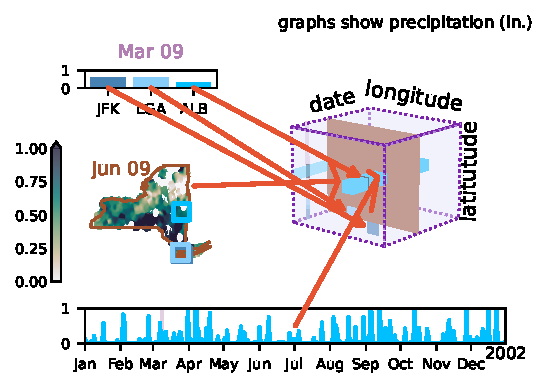
\includegraphics[width=3.5in, alt={Data cube illustrating index space with map, timeseries, and bar charts visualizing slices of the data.}]{k_different_types.pdf}
\end{center}
\caption{This weather station data has multiple embedded continuities - points at each time and position, timeseries at each position, and maps at each time - that are expected to be homeomorphic to the continuity of their respective visualizations.}
    \label{fig:homeomorphism}
\end{figure}

For example, a \texttt{line} algorithm often does not have a way to query whether a list of (x,y) coordinates is the distinct rows, the time series, or the list of stations in \autoref{fig:homeomorphism}. We propose that the bar plot, line plot, and heatmap can be verified as structure preserving because they have a homeomorphic relationship to the 0D ($\bullet$) points, 1D (--) linear, and 2D ($\blacksquare$) surface continuities embedded in the continuous 3 dimensional. Our methodology generalizes Bertin\cite{bertinSemiologyGraphicsDiagrams2011}'s codification of structure,  Mackinlay's\cite{mackinlayAutomaticDesignGraphical1987} mathematical formalization, Wilkinson's set theoretic approach \cite{wilkinsonGrammarGraphics2005}, and Kindlemann and Scheidegger's algebraic visualization design (AVD) framework \cite{kindlmannAlgebraicProcessVisualization2014} by explicitly incorporating topology, supporting non-group and non-monoidal structures, and providing a framework for translating the theoretical ideas into buildable components.

Throughout this paper we will be discussing visualization primarily, but by changing the last of the three fiber bundles (the graphic bundle) we discuss in Section~\ref{sec:data models}, we could go from a visual representation to an auditory, haptic, or any other modality and retain the benefits we identify from the fiber bundle and sheaf structures.

\section{Data Model}
\label{sec:data models}

\begin{table}[!h]
  \caption{Summary of how the data is abstracted using topological structures}
  \label{tab:data_abstraction}
  \centering
  \scriptsize
  \begin{tabu}{|r | l l l l|}
    \hline
    &\textcolor{base}{point}/\textcolor{base}{openset}/\textcolor{base}{base} & \textcolor{fiber}{fiber} & \textcolor{total}{total} & Fiber bundle\\
     &  index/subset/indices & record/fields &  data type & \\
    \hline
   Data & $\dbasepointc \in \opensetc \subseteq \dbasec$ & $\delementc \in \dfiberc$ & \dtotalc &  $\dfiberc \hookrightarrow \dtotalc \rightarrow \dbasec$  \\
   Visual & $\dbasepointc \in \opensetc \subseteq \dbasec$  & $\velementc \in \vfiberc$ & \vtotalc & $\vfiberc \hookrightarrow \vtotalc \rightarrow \dbasec$\\
   Graphic & $\gbasepointc \in \opensetgc \subseteq \gbasec$ & $\gelementc \in \gfiberc$ & \gtotalc &$\gfiberc \hookrightarrow \gtotalc \rightarrow \gbasec$ \\
   \hline
  \end{tabu}
\end{table}

We model data as a fiber bundle because it can encode topological properties, field types, and data values in a uniform manner.  We extend Butler's proposal of using fiber bundles as an abstraction for visualization data \cite{butlerVectorBundleClassesForm1992,butlerVisualizationModelBased1989} by incorporating Spivak's fiber bundle representation of relational databases \cite{spivakDatabasesAreCategories2010,spivakSimplicialDatabases2009}. As we show in Table~\ref{tab:data_abstraction} and Table~\ref{tab:data_sheaves}, where Spivak represents a database schema with the bundle's fiber space \dfiber\, topological indexing through a base space \dbase\, and a specific dataset as a section of the bundle \dsection\, and we introduce parallel analogous structures representing visual and graphic specifications.

\begin{figure}[!h]
    %\begin{multicols}{2}
    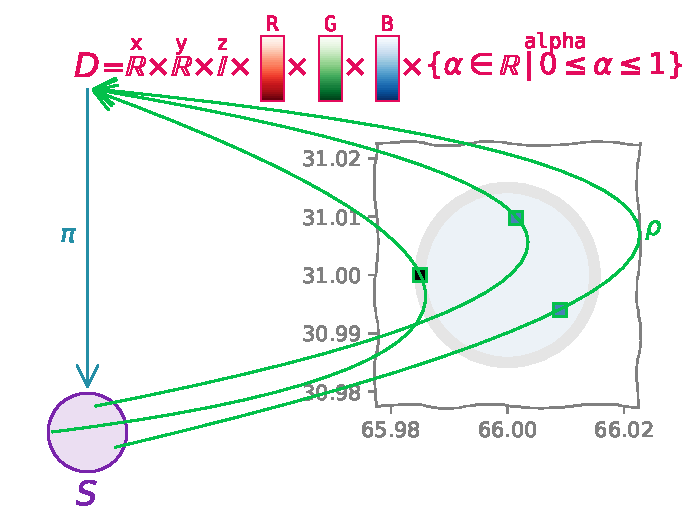
\includegraphics[width=.5\textwidth, alt={illustration of how a pixel in a scatter plot is the return value of a function from the graphic indexing space to the fiber space that specifies the display space}]{fb_rho.pdf}
%    \columnbreak
    \caption{The scatter marker is specified by the section $\gsection$, which maps from a point $\gbasepoint \in \gbase$ into the fiber $\gfiber$ to retrieve the values that compose into the pixel (approximated as a square). The section evaluated over the entire space $\gsection\vert_{S}$ returns the entire scatter mark, shown here in faded form to make it easier to see the individual pixels.}\label{fig:fiber_bundle}
\end{figure}


By choosing a topological space $\mathcal T$ as indexing space underlying the dataset we get a uniform abstraction for describing arbitrary continuity -- time series, lists of observations, spatial fields all have the same abstract structure -- and we get a method for managing overlapping embedded topologies, such as we show in \autoref{fig:homeomorphism}. Spivak's fiber bundle construction of types decouples field types from field names and single-dimensional and multi-dimensional fields share a common abstraction: they all rely on some choice of mathematical object for the data types. A particular dataset can in this paradigm be encoded as a \textcolor{section} \dsectionc\ of a bundle, assigning to each index value an observation in the data types prescribed by the fiber space. This fits topology and field types into a data definition $\textcolor{section}{\texttt{dataset}}: \textcolor{base}{\texttt{topology}} \rightarrow \textcolor{fiber}{\texttt{field}}$. We abstract these data containers as sheaves $\sheafc$, as summarized in \autoref{tab:data_sheaves} and the gluing property of sheaves provides a systematic way to track continuity of the data \cite{ghristElementaryAppliedTopology2014} and apply visual algorithms developed on this model regardless whether the data fits in memory, is distributed, or streaming.

\begin{table}
  \caption{Functions that associate topological subspaces with records}
  \label{tab:data_sheaves}
  \centering
   \scriptsize%
  \begin{tabu}{|r | l l | }
    \hline
     & \textcolor{section}{section} & \textcolor{sheaf}{sheaf} \\
     & record at location & set of possible records for subset \\
     \hline
  Data & $ \cgamma{\dbasec}{\dtotalc} \ni \dsectionc: \dbase \textcolor{section}{\rightarrow} \dfiberc$ & $\sheafc_{\dbasec, \dtotalc}: \opensetc \rightarrow \cgamma{\opensetc}{\dtotalc\restriction_{\opensetc}}$\\
  Visual &  $\cgamma{\dbasec}{\vtotalc} \ni \vsectionc: \dbase \textcolor{section}{\rightarrow} \vfiberc$ & $\sheafc_{\dbasec, \vtotalc}: \opensetc \rightarrow \cgamma{\opensetc}{\vtotalc\restriction_{\opensetc}}$\\
  Graphic &    $\cgamma{\gbasec}{\gtotalc} \ni \gsectionc: \gbase \textcolor{section}{\rightarrow} \gfiberc$ &  $\sheafc_{\gbasec, \gtotalc}: \opensetgc \rightarrow \cgamma{\opensetc}{\gtotalc\restriction_{\opensetgc}}$ \\
  \hline
  \end{tabu}
\end{table}

\section{Artist}
\label{sec:Artist}

We call the mapping from data to graphic $\vartistc:\dsectionc\mapsto\gsectionc$ an \textcolor{artist}{Artist}. Artists are named for the artist class in Matplotlib because the Artist class (and its children) assemble and manage the visual
elements produced in Matplotlib\cite{hunterArchitectureOpenSource}. We propose that Artists (the transform and the library implementation) are structure preserving when they are implemented as sheaf maps from the data representation sheaf to the graphics sheaf. This means that the artist satisfies the following constraints, as illustrated in \autoref{fig:artist}:

\begin{figure}[!h]
    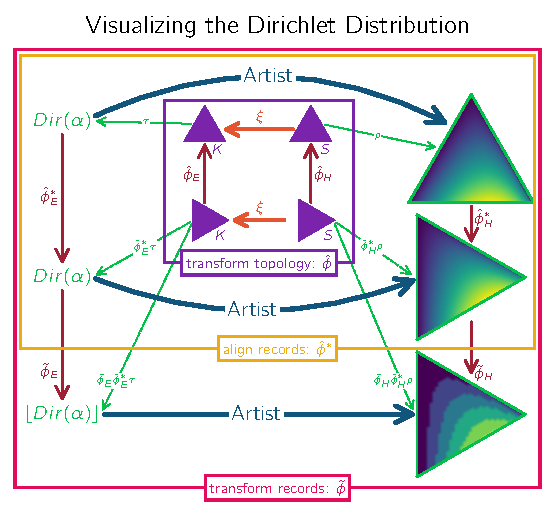
\includegraphics[width=.5\textwidth, alt={Diagram of a dirichelet distribution evaluated on a triangle, transposed, and binned and the corresponding visualization output by the artist function.}]{artist_equiv.pdf}
    \caption{The transposition of the Dirichilet distribution is preserved in the visualization because the Artist implements presheaf constraints and the binning of the Dirichelet data is preserved in the visualization because the artist is equivariant.}\label{fig:artist}
\end{figure}

\begin{description}
    \item[homotopic] there exists a deformation retract\footnote{A deformation retract is required because it ensures a continuous mapping between graphic and data continuity when a screen is 2-dimensional and the data continuity is <2D]} $\vindexc: \gbasec\rightarrow\dbasec$ between graphic and artist base space
    \item[topology] the artist is commutative w.r.t. the presheaf morphism $\dfunchc: \dbasepointc^{\prime}\mapsto \dbasepointc$ and pullback $\dfuncpullc \dsectionc \restriction_{\opensetc^{\prime}}: \dsectionc\restriction_{\opensetc^{\prime}} \mapsto \dsectionc \restriction_{\opensetc^{\prime} \circ \dfunchc}$: index changes on the record leave values in the record unmodified
    $\dsectionc(\dbasec) = \dfuncpullc\dsectionc(\dbasepointc^{\prime}) = \dsectionc(\dfunchc(\dbasepointc^{\prime}))$
    \item[fields] the artist is commutative w.r.t. actions on the fiber. An action $\dfunctc: \dfiberc\to\dfiberc$ induces a function between sections $\dfunctc: \dfuncpullc \dsectionc \restriction_{\opensetc^{\prime}} \mapsto \dfuncpullc \dsectionc^{\prime} \restriction_{\opensetc}$. We also require $\dfunctc$ to respect the structure, such as operators, of $\dfiberc$.
\end{description}

With this underlying topological structure to describe the visualization pipeline, traditional constructions from topology and category theory generate natural operators on the data structures.
\begin{figure}[!h]
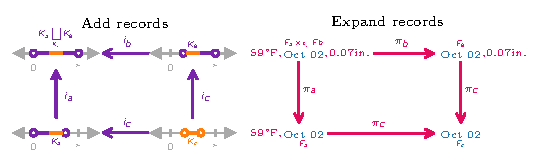
\includegraphics[width=3.5in, alt={Records are added by taking the union of base spaces. Fields are added by taking the cartesian product of fiber spaces.}]{more_records.pdf}
\caption{Pullback (left) and pushout (right) structure of the operations that add records (increasing the indexing base space) or expand records (merging different fiber spaces with a database join-like operation).}\label{fig:more-records}
\end{figure}

Pushouts and pullbacks, of central importance in category theory and topology, emerge here as operators to add and extend records, respectively. Since (in categorical language) sheaf maps preserve limits and colimits, this observation shows that artists are composable: $\vartistc(\bigsqcup\limits_{i}\dbasec_i, \prod\limits_j\dfiberc_j) = \bigsqcup\limits_i\prod\limits_j\vartistc(\dbasec_i, \dfiberc_j)$




\begin{figure*}[h]
    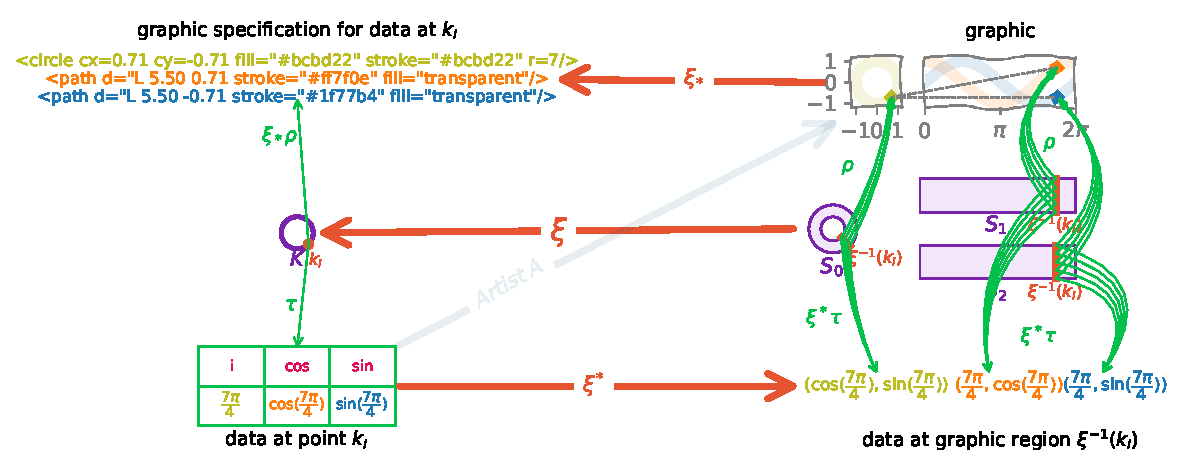
\includegraphics[width=7.16in, alt={An annulus indexing space deformation retracts into a circle. For any point i, cos(i), sin(i), there is a specification to draw a piece of a circle, sine plot, and cosine plot, a  patch of pixels of a rendered circle, sin plot, and cosine plot. Hovering over any of those pixels should get back the data i, cos(i), sin(i)}]{xi_diagram.pdf}
    \caption{A deformation retract $\vindexc$ that relates the graphics footprint $S_0$ of an abstract circle to the circle itself gives rise to a pair of additional maps. The pushforward $\vindexpushc$ matches a point in the graphical realization to the specification of the graphic at that point, while the pullback $\vindexpullc$ matches each point in the graphic space to the data giving rise to that point.
    }
    \label{fig:xi}
\end{figure*}

As illustrated in \autoref{fig:xi}, this deformation retract $\vindexc$ gives rise to two so-called transport functors $(\vindexpush, \vindexpull)$ -- known as the pushforward $\vindexpushc$ and pullback\footnote{different use of the word pullback than in the preceding paragraph -- an unfortunate collision of terminology} $\vindexpullc$. These functors also codify how visual elements correspond to distinct data elements, which is a necessary condition of a visualization being readable\cite{ziemkiewiczEmbeddingInformationVisualization2009}. The pushforward $\vindexpushc$ matches each point in the data space to the specification of the graphic at that point $\vindexpushc\gsectionc(\dbasepointc) = \gsectionc\restriction_{\vindexprec(\dbasepointc)}$, while the pullback $\vindexpull$ matches each point in the graphic space to the data over that point $\vindexpullc\dsectionc(\gbasepointc) = \dsectionc(\vindexc(\gbasepointc)) = \dsectionc(\dbasepointc)$. If the map $\vindex$ was explicitly implemented with the corresponding sheaves, the information in $\dsection, \vindexpull\dsection,\gsection, \vindexpush\gsection$, as illustrated in \autoref{fig:xi}, could be exposed to an accessibility tool (like a screen reader). This functionality could, for example, compensate for a major accessibility limitation of the current Matplotlib architecture, which is that the interactive widgets and GUIs are rendered as PNGs (so that Matplotlib does not have to maintain a GUI library) which means that screen readers cannot query the individual elements.

\section{Construction}
\begin{figure}[!h]
  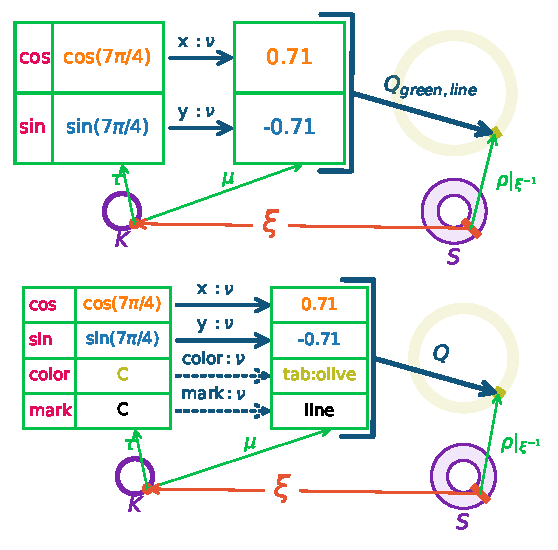
\includegraphics[width=1\columnwidth, alt={cos(i) and sin(i) gets encoded as x and y values that for a patch of a green circle. That the visual mark is a green line can either be encoded in the compositor function or passed to the compositor function as part of the encoding spec. Green and line can be pulled back to represent constant parameters of the data.}]{construction.pdf}
  \caption{The compositor $\vmark$ can be fully specified $\vmark_{green,line}$ such that the only input is the encoding of the data values. Alternatively, the compositor $\vmark$ supports more customizability by encoding  a constant parameters in the visual bundle, which pulls back to constant parameters in the data bundle.}\label{fig:construction:q}
\end{figure}

Artists naturally factorize into a two-stage process, starting with an encoding stage $\vchannelc$ followed by a compositing stage $\vmarkc$.
In the \textcolor{artist}{encoding} stage $\vchannelc$, a data bundle is mapped to a visual variable bundle \vchannel. Since $\dtotal$ and $vtotal$ are structurally identical, any $\vtotal$ can be redefined as $\dtotal$; therefore, as shown in \autoref{eq:construction:nu:fabrication}, any collection of $\vchannel$ functions can be composed such that they are equivalent to a $\vchannel$ that directly converts the input to the output.
\begin{equation}
  \label{eq:construction:nu:fabrication}
  \begin{tikzcd}
    \dfiberc_{\dbasepointc}
    \arrow[rr, "\vchannelc", color=artist]
    \arrow[rrrr, "\vchannelc^{\prime\prime}", dashed, bend right, color=artist] &  &
    \vfiberc_{\dbasepointc}\coloneqq{\dfiberc_{\dbasepointc}^{\prime}}
    \arrow[rr, "\vchannelc^{\prime}", color=artist] &  &
    \vfiberc^{\prime}_{\dbasepointc}
  \end{tikzcd}
\end{equation}

 As with artists, $\vchannel$ are maps of sections such that operators can also act on transformers $\vchannel$, meaning that encoders can be added $\vchannel_{a+b} = \vchannel_{a} + \vchannel_{b}$ and multiplied d $\vchannel_{a\times b} = \vchannel_{a}  \vchannel_{b}$.


\begin{table}[!h]
  \centering
  \begin{tabulary}{\columnwidth}{|l|L|l|}\hline
   \(\bm{\vchannel_{i}}\)    & \(\bm{\vsection_{i}}\)  & \(\bm{codomain(\vchannel_{i}) \subset \vfiber_{i}}\)  \\ \hline
  position                    & x, y, z, theta, r      & \(\mathbb{R}\)   \\ \hline
  size                        & linewidth, markersize  & \(\mathbb{R}^{+}\)  \\ \hline
  shape                       & markerstyle            & \(\{f_{0}, \ldots, f_{n}\}\)\\ \hline
  color                       & color, facecolor, markerfacecolor, edgecolor  & \(\mathbb{R}^{4}\) \\ \hline
  \multirow{2}{*}{texture}    & hatch      & \(\mathbb{N}^{10}\)\\\cline{2-3}
                              & linestyle    & \((\mathbb{R}, \mathbb{R^+}^{n, n\%2=0})\) \\ \hline
  \end{tabulary}
  \caption{Some of the $\vfiber$ components of the $\vtotal$ bundles in Matplotlib components}
  \label{tab:math:artist:mpl:fiber}
\end{table}

The fibers of \vchannel\ are an internal library specification of graphics. For example, \autoref{tab:math:artist:mpl:fiber} shows a standardized internal representation of the visual parameters used by Matplotlib functions. One of the ways Matplotlib facilitates accessibility is by allowing the user to customize most of the aesthetics - colors, fonts, textures. Standardizing the internal parameters provides for a consistent interface for external accessibility tools, such as libraries of accessible stylesheets or tools that may want to query the Matplotlib Artist for context of the current state.

The \textcolor{artist}{compositing} stage $\vmarkc$ then assembles the visual components into a visual element. Since encoder functions are infinitely composable, as described in \autoref{eq:construction:nu:fabrication}, a new compositor function $\vmarkc$ can be constructed by pre=composing $\vchannelc$ functions with the existing $\vmarkc$.
\begin{equation}
  \label{eq:construction:q:fabrication}
  \begin{tikzcd}
      \cgamma{\dbasec}{\vtotalc}
      \arrow[rr, "\vchannel", color=artist]
      \arrow[rrrr, "\vmarkc^{\prime}", bend right, color=artist, dashed] &  & \cgamma{\dbasec}{\vtotalc^{\prime}}
      \arrow[rr, "\vmarkc", color=artist] &  & \cgamma{\gbasec}{\gtotalc}
      \end{tikzcd}
\end{equation}
The composition in \autoref{eq:construction:q:fabrication} means that different measurable components can yield the same visual elements. Operators can also act on compositors $\vmark$ such that $\vmark_{a+b} = \vmark_{a} + \vmark_{b}$ and multiplied d $\vmark_{a\times b} = \vmark_{a}  \vmark_{b}$.

\begin{figure}[!h]
  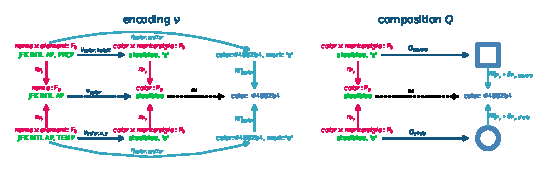
\includegraphics[width=\columnwidth, alt={The data value JFK INTL AP is paired with different variables (pressure and temperature) to verify that JFK is consistently encoded as the same color while pressure and temperature are encoded as different marker styles. The markerstyles and colors are then tested to ensure that the compositor builds a square and a circle that are the same color.}]{nu_qu.pdf}
  \caption{The composability of the model allows for separation of concern in testing: the encoding functions $vchannel$ are tested to ensure that they convert the data into the internal specification, while the compositors are tested to ensure that the visual specifications are encoded consistently.}\label{fig:construction:verification}
\end{figure}
As illustrated in \autoref{fig:construction:verification}, the factorization of the artist into the encoding and composition stages provides a framework for testing each independently. For example, encoders build in this framework would be designed to ensure that a transformation from a non colorblind safe colormap into a colorblind safe colormap would ensure that the colormaps are equivalent such that the transformation is not introducing a change in structure. Similarly, the composition stage can be tested to ensure that parameters are applied consistently across visual elements and, as with encoding, more accessible elements can be swapped in without introducing new structure.


\section{Conclusion}

We have demonstrated a mathematical formalism for representing the architecture of components in a data visualization library, in which the mathematical structures both enforce well known principles of data visualization and suggest factorizations and decompositions the result in highly modularizable infrastructure, such that artists can be constructed from composable primitive. This decomposability leads directly to a test framework ambition: if we can split $A=\vmarkc\circ\vchannelc$, and each factor $\vchannelc$, $\vmarkc$ can be further decomposed into composable primitives, we can focus testing on each of these building blocks reducing testing for correctness of the process as a whole to correctness of each building block, and correctness of their chosen combinations. The composability of this framework allows for staged adaptation such that it can be incorporated into an existing library, as exemplified by \url{https://github.com/matplotlib/data-prototype}. Furthermore, while the graphics sheaves here deal with visual properties -- pixel positions and colors, et.c. -- one could easily imagine picking a different choice for the fiber $\gfiberc$ in the realization sheaf that tracks information about haptic or auditory expressions, resulting in an identical abstraction, with many overlapping building blocks, for multimodal data representations.


\section*{Supplemental Materials}
\label{sec:supplemental_materials}
This paper reuses figures from a longer version of this paper; therefore all code for the figures can be found in \url{https://github.com/story645/team/paper/figcode}. Additionally, there is an attached supplement with a glossary of math terms used in this paper.

\section*{Acknowledgements}
The authors would like to thank the anonymous reviewers who gave constructive feedback on an earlier version of this paper. The authors are also grateful to  the various Matplotlib and Napari contributors, particularly Juan Nunez-Iglesias, and Nicolas Kruchten for their valuable feedback from the library developer perspective. Hannah is also very grateful to Nicolas for the suggestion of augmented notation and to the nlab and wikipedia contributors who wrote clear explanations of many of the topics discussed in this paper. This project has been made possible in part by grant number 2019-207333 (EOSS Cycle 1) and EOSS Cycle 3 Chan Zuckerberg Initiative DAF, an advised fund of Silicon Valley Community Foundation


\bibliographystyle{plain}
\bibliography{references}
\end{document}
